% !TEX root = master_thesis.tex
\chapter{Discussion}
\label{chap:disc}
This chapter will present a discussion of results for the beam asymmetry $\Sigma$ in the reaction $\gamma p \to p\eta'\to p\gamma\gamma$ obtained with the CBELSA/TAPS experiment. No dedicated discussion of the results obtained for $\eta$ photoproduction will be given here. Very good agreement between the results for $\Sigma_\eta$ in this work and reference \cite{farahphd} makes this obsolete, because the findings for $\Sigma_\eta$ compared to various previous measurements and existing PWA predictions are discussed in reference \cite{farahphd} in detail. However, final remarks regarding the used fitting methods will be made after the results for $\Sigma_{\eta'}$ obtained in this thesis were compared to existing data, and as a next step compared to existing PWA model predictions. 
\section{Comparison of results to existing data}
The data situation for any observables in $\eta'$ photoproduction is scarce because on one hand the production cross section is very small while on the other hand high center of mass energies are needed to observe the reaction $\gamma p \to p\eta'$ \cite{pdg}.  To collect sufficient statistics at these energies, very high energetic photon beams are necessary because the photon beam Intensity $I(E_\gamma)$ approximately behaves like \cite{leo}
\begin{equation}
	I(E_\gamma)\propto\frac{1}{E_\gamma}.
	\label{eq:int}
\end{equation} 
Next to a measurement of the beam asymmetry in $\eta'$ photoproduction near threshold at GrAAL \cite{thresh}, there exists one other recent measurement of $\Sigma_{\eta'}$ at CLAS \cite{collins}. In this work the beam asymmetry could be extracted covering the beam energy range of $\SI{1500}{\mega\eV}\leq E_\gamma<\SI{1800}{\mega\eV}$ and is binned as $\left(\Delta E_\gamma,\Delta\cos\theta\right)=\left(\SI{100}{\mega\eV},0.33\right)$ . Thus, only the results from reference \cite{collins} are suited for comparison which are binned as $\left(\Delta E_\gamma,\Delta\cos\theta\right)=\left(\SI{54}{\mega\eV},0.2\right)$. Of all kinematic bins provided by reference \cite{collins} only energy bins where the bin centers approximately align with the energy bins chosen in this thesis are considered for further investigation .
Figure \ref{fig:etapcollins} shows the results for the beam asymmetry $\Sigma_{\eta'}$ compared with results reported by \cite{collins}.
\begin{figure}[htbp]
	\centering
	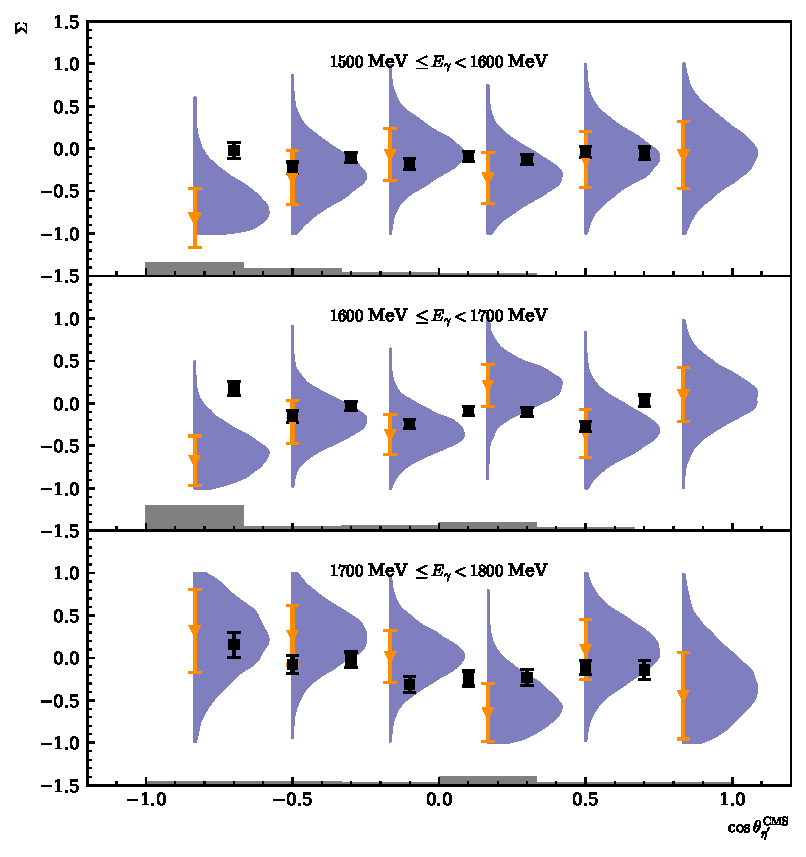
\includegraphics[width=\linewidth]{../bayes/etap_event_based_fit/plots/sigma_etap_data.pdf}
	\caption{Results for the beam asymmetry $\Sigma_{\eta'}$ (orange errorbars and distributions) compared with the results for the energy bins $E_\gamma=\SI{1569}{\mega\eV},E_\gamma=\SI{1676}{\mega\eV},E_\gamma=\SI{1729}{\mega\eV}$ reported in reference \cite{collins} (black errorbars).   Systematical errors are shown as grey bars.}
	\label{fig:etapcollins}
\end{figure}
First of all, one may notice the large difference in statistical errors between the two datasets. This can be explained by considering that the results obtained by \textsc{Collins et al.} \cite{collins} were extracted via the charged decay $\eta'\to\pi^+\pi^-\eta\to2\pi^+2\pi^-\pi^0$ with a branching ratio of $\text{BR}=42.6\cdot22.02\%=9.38\%$ \cite{pdg} as opposed to the neutral decay $\eta'\to\gamma\gamma$ with a branching ratio of $\text{BR}=2.2\%$ \cite{pdg}. Furthermore, the electrons impinging on the radiator target at CLAS were accelerated to  $\SI{4.5}{\giga\eV}$ \cite{collins}, increasing the statistics in the photon beam energy range of interest compared with CBELSA/TAPS data, where the electrons are only accelerated to  $\SI{3.2}{\giga\eV}$. Aside from the large difference in statistical errors, generally good agreement between the two datasets exists. Most datapoints are compatible within their statistcal errors and the angular profile of the beam asymmetry is displayed equivalently. The largest discrepancy between both datasets exists in backwards direction for the first two energy bins;  although the angular bins do not exactly match it is noteworthy that there is a sign flip between the different measurements that can not be accounted for by combined statistical and systematical error (for the CLAS measurement a systematic error due to the determination of the photon beam polarization of $6\%$ is reported \cite{collins}). It is not understood why these bins show this particular behavior as no indication towards any additional systematic effects has been found. Note however that without identical binning only vague conclusions regarding the agreement of both datasets can be made. The given datasets allow to identify that there is in general consistency and no large unaccounted systematic uncertainties. Direct comparibility can only be achieved if statistics at high center of mass energies are increased at the CBELSA/TAPS experiment. 

Due to the placement of the coherent edge the beam asymmetry $\Sigma_{\eta'}$ could be extracted at beam energies up to $E_\gamma=\SI{1800}{\mega\eV}$ in this work although the CBELSA/TAPS experiment theoretically provides photon beam energies of maximally $E_\gamma^\text{max}=\SI{3200}{\mega\eV}$. Yet, the event yield included less than $10^4$ $\gamma p\to p\eta'\to p\gamma\gamma$ events in the selected energy region collected in roughly four months of beam time. The beam asymmetry in $\pi^0$($\eta$) photoproduction in reference \cite{farahphd} was determined using $6.28\cdot10^6$($5.24\cdot10^5$) events giving significantly higher precision. Next to small cross section and branching ratio to a neutral final state this illustrates the effect of Eq. \ref{eq:int} during data collection leading to large statistical errors and background contributions when determining the beam asymmetry. Furthermore only a coarse binning in $\left(E_\gamma,\cos\theta\right)$ could be chosen to account for the available statistics, denying a detailed investigation of the beam asymmetry $\Sigma_{\eta'}\left(E_\gamma,\cos\theta\right)$. In order to collect more statistics at high beam energies in future beam times of the CBELSA/TAPS experiment, e.g. to further investigate the reaction $\gamma p\to p\eta'$, either longer beam times and/or shifting the coherent edge towards higher energies should be considered. Also the decay channel $\eta'\to\pi^0\pi^0\eta$ may be investigated to increase precision of the existing data. The use of machine learning methods to identify background contributions during event selection \cite{ml} could also allow a more precise measurement of the beam asymmetry $\Sigma_{\eta'}$.
\section{Comparison of results to PWA calculations}
Figure \ref{fig:pwa} shows the new results for the beam asymmetry $\Sigma$ in $\eta'$ photoproduction obtained with the CBELSA/TAPS experiment compared with existing PWA-predictions. Shown is the etaMAID2018 solution \cite{etaMAID}, as well as the Bonn-Gatchina (BnGa) solution \cite{etap_bnga} which already include results from the measurements \cite{collins} and \cite{thresh} in the fit. This however puts bias towards  the fitted data on the PWA solution such that the same remarks regarding agreement of the results of this thesis and the PWA calculations can be made as in the previous section; generally the obtained data points are described well by the PWA predictions with the exception of the backwards direction at the first two energy bins. This indicates that the previous measurements of $\Sigma_{\eta'}$ had a large influence on the PWA fits, especially when considering that before these measurements were added, the PWA solutions failed to describe the beam asymmetry in $\eta'$ photoproduction, generally showing the wrong sign \cite{collins}. Thus, similarly to the previous section, only a vague conclusion of general agreement between data points and PWA solutions can be drawn. Further measurements are required to increase the precision of existing PWA models. Following the suggestions of \textsc{Tiator et al.} \cite{etaMAID} more observable measurements are especially needed near the $\eta'$ production threshold to resolve discrepancies between different PWA solutions. It is hereby crucial to measure with high precision in small energy bins. In addition to more precise measurements of the differential cross section and the beam asymmetry near threshold the observables $T$ and $F$ could be measured as a next step to improve the quality of the PWA solutions \cite{etaMAID}. Figure \ref{fig:pwas} shows all 8 single and double polarization observables near threshold as predicted by different resonance contributions of the etaMAID \cite{etaMAID} (red lines) and Bonn-Gatchina \cite{etap_bnga} (black lines) PWA groups. It is evident that the measurements of additional observables will help to eliminate ambiguities in the future.
\begin{figure}[htbp]
\centering
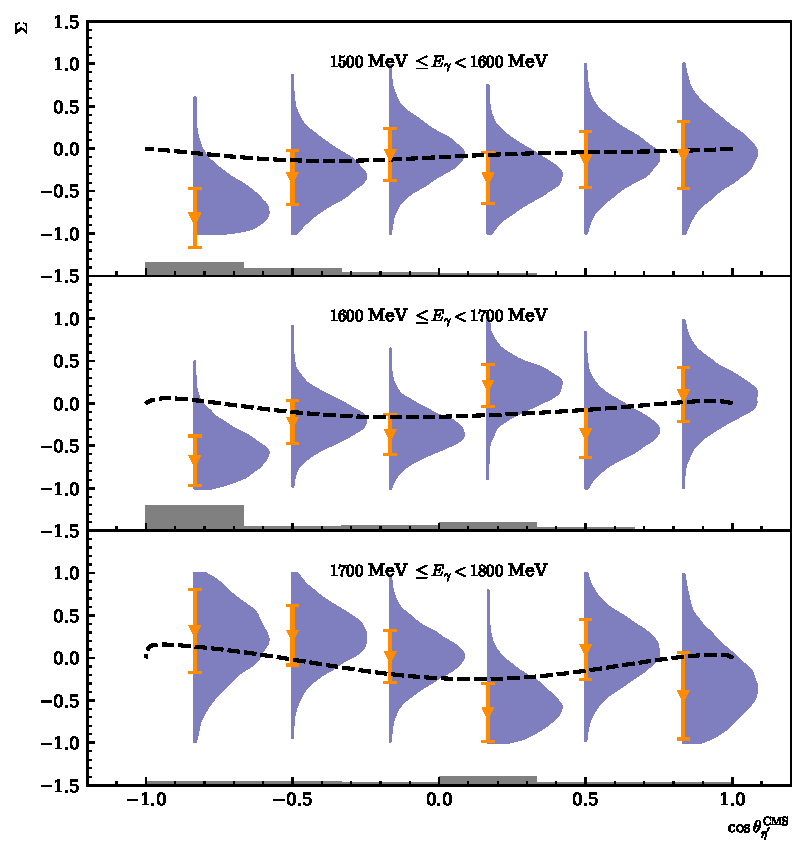
\includegraphics[width=\linewidth]{../bayes/etap_event_based_fit/plots/sigma_etap_pwa.pdf}
\caption{Results for the beam asymmetry $\Sigma_{\eta'}$ (orange errorbars and distributions) compared with PWA solutions:  etaMAID \cite{etaMAID,pwa_online} (dashed black line) and BnGa \cite{etap_bnga} (dashed red line). The errorbars only depict statistical error, the systematic error is shown as grey bars.}
\label{fig:pwa}
\end{figure}

\begin{figure}[htbp]
	\centering
	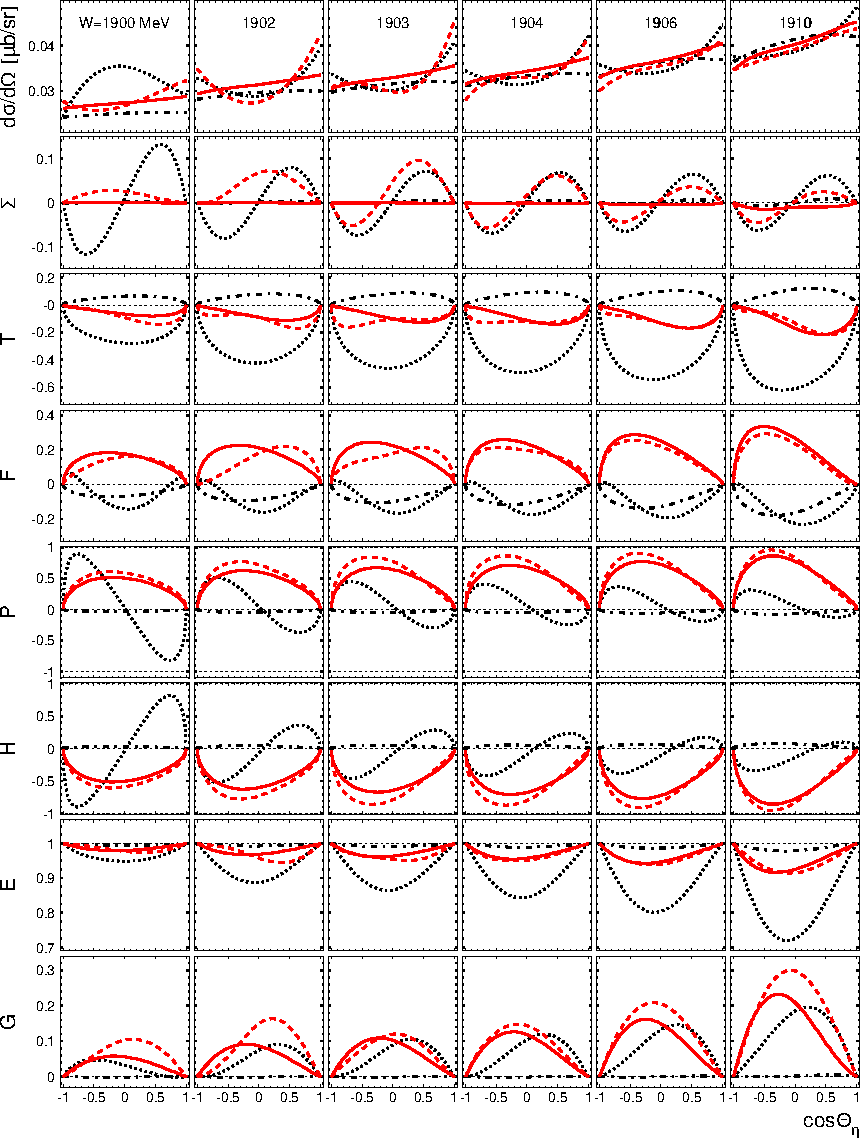
\includegraphics[width=\linewidth]{pwas}
	\caption{Different resonance contributions to all eight single and double polarization observables as predicted by etaMAID \cite{etaMAID} and Bonn-Gatchina \cite{etap_bnga} PWA solutions near the $\eta'$ production threshold. Taken from \cite{etaMAID}.}
	\label{fig:pwas}
\end{figure} 
\section{Final discussion of methods}
Next to acquiring new data for the beam asymmetry $\Sigma$ in the reaction $\gamma p\to p\eta'$ the main focus of this thesis laid in the exploration of alternative fitting methods using \textsc{Bayesian} statistics. A final r\'{e}sum\'{e} is now drawn here with regard to the different strategies used to extract the beam asymmetry $\Sigma$ in this work.

First tests of the \textsc{Bayesian} approach were performed when confirming already published results for the beam asymmetry in $\eta$ photoproduction \cite{farahphd,eta} and were successively also applied to data obtained from $\eta'$ photoproduction. Two methods of extracting $\Sigma$ were discussed;

The combination of normalized event yields into the asymmetry (see section \ref{subsec:evyield})
	\begin{equation}
		A(\phi)=\frac{\tilde{N}^\bot-\tilde{N}^\parallel}{p_\gamma^\parallel\tilde{N}^\bot+p_\gamma^\bot\tilde{N}^\parallel}=\Sigma\cos\left(2\left(\alpha^\parallel-\phi\right)\right).
	\end{equation} 
allowed to determine the beam asymmetry as a fit parameter for each kinematic bin. Without introducing systematic error the fit could be performed either as a least squares fit or a \textsc{Bayesian} fit. The former resulting in a point estimate with statistical errors $\hat{\Sigma}\pm\sigma_{\hat{\Sigma}}$, the latter resulting in a marginal posterior distributions $p\left(\Sigma|y\right)$ and both fits were able to give a measure of goodness of fit. It was shown that the obtained statistical error bars provide the width of a $1\sigma$ interval of the 
marginal posteriors, indicating that both approaches are indeed equivalent. The implementation of the \textsc{Bayesian} fit did not require unreasonably more effort compared to the implementation of a $\chi^2$-fit, mainly due to the neat structure of the used programming language Stan \cite{stan}. Computation time of the \textsc{Bayesian} fit exceeded the time needed for a $\chi^2$ fit but not significantly. Nevertheless the nature of MCMC fits required diagnosing the convergence of the fit itself carefully, in total making the \textsc{Bayesian} approach more elaborate without increasing the knowledge gained from the fit results significantly because the posteriors are without exception unimodal \textsc{Gaussians}, when they are not truncated by the upper or lower bound for $\Sigma$. Yet, any deviations from unimodal \textsc{Gaussian} posteriors \emph{could} be revealed by using the \textsc{Bayesian} approach that also provides great flexibility when using the results as input for PWA calculations. The most important conclusion to be drawn is that a \textsc{Bayesian} approach is valid and produces the same results as the so far pursued approach of least-squares fitting because creating the same results with different independent methods naturally increases their informative value. However, because the binning of data introduces systematic under- or overestimation of the fit parameter $\Sigma$ (cf. appendix \ref{app:binnedfits}) determining the beam asymmetry from the quantity $A\left(\phi\right)$ should be avoided.

The second method that was used to extract the beam asymmetry was an unbinned fit using the likelihood (see section \ref{subsec:evfit})
\begin{equation}
	\begin{aligned}
		\ln\mathcal{L}&=\sum_{i=1}^{n}\ln p_\text{prompt}\left(\phi_i,p_{\gamma,i}\big|\Sigma,a,b,\Sigma^\text{bkg},a^\text{bkg},b^\text{bkg}\right)\\&+\sum_{j=1}^m \ln p_\text{sideband}\left(\phi_j,p_{\gamma,j}\big|\Sigma^\text{bkg},a^\text{bkg},b^\text{bkg}\right).
	\end{aligned}
\end{equation}
The frequentist approach aimed to estimate all parameters with statistical errors by maximizing this likelihood while in a \textsc{Bayesian} approach it was embedded into a full probabilistic model, leading to a complete inference for all parameters. Both methods lack a measure of goodness of fit so that toy Monte Carlo experiments were needed to confirm the right working principle which were conducted successfully without revealing bias or sources of systematic errors. Again, the two approaches are found to be equivalent, as estimated from the widths of the distributions and the statistical errors of the point estimates. The same remarks regarding the implementation and interpretation of the two fits as before apply, however computation time for the unbinned \textsc{Bayesian} is now significantly larger. While the unbinned maximum likelihood fit takes seconds, for specific kinematic bins the unbinned \textsc{Bayesian} fit took up to 20 minutes. Applying the \textsc{Bayesian} approach to data selected in the frame of this thesis for the reaction $\gamma p\to p\eta'\to p\gamma\gamma$ furthermore revealed the great advantage of the flexibility fully \textsc{Bayesian} models provide; since a significant amount of background reactions from $2\pi^0$ production is part of the selected data, this had to be considered when determining the beam asymmetry. For the maximum likelihood fit the point estimates had to be shifted \emph{after} the fit, depending on the amount of background. For the \textsc{Bayesian} fit however background contributions could be included inherently into the likelihood function, allowing to extract the corrected distributions directly from the fit.

In summary, one can say that the application of \textsc{Bayesian} methods when extracting the polarization observable $\Sigma$ was successful. Equivalence to frequentist methods was shown while at the same time the \textsc{Bayesian} fits provide more flexibility and the possibility to investigate the structure of posterior distributions. 
